% This is LLNCS.DEM the demonstration file of
% the LaTeX macro package from Springer-Verlag
% for Lecture Notes in Computer Science,
% version 2.4 for LaTeX2e as of 16. April 2010
%
\documentclass{llncs}
%
%\usepackage{ctex}
\usepackage{CJKutf8}
\usepackage{graphicx}
\usepackage{makeidx}  % allows for indexgeneration
\usepackage{amsmath}
\begin{document}
%
%\frontmatter          % for the preliminaries
%
%\pagestyle{headings}  % switches on printing of running heads

%\addtocmark{Hamiltonian Mechanics} % additional mark in the TOC

%
%\mainmatter              % start of the contributions
%
\title{A Distance-Based Scoring Method
for Document-Based Question Answering}
%
\titlerunning{A Distance-Based Scoring Method}  % abbreviated title (for running head)
%                                     also used for the TOC unless
%                                     \toctitle is used
%
\author{Liansheng Lin\inst{1} \and Han Ni\inst{2} \and Ge Xu\inst{3}}
%
%\authorrunning{Ivar Ekeland et al.} % abbreviated author list (for running head)
%
%%%% list of authors for the TOC (use if author list has to be modified)
%\tocauthor{Ivar Ekeland, Roger Temam, Jeffrey Dean, David Grove,
%Craig Chambers, Kim B. Bruce, and Elisa Bertino}
%
\institute{Fuzhou University, Fuzhou, China \\
\email{linliansheng@nd.com.cn}
\and NedDragon Websoft Inc., Fuzhou, China \\
\email{ni.han.ms6@foxmail.com}
\and Minjiang University, Fuzhou, China \\
\email{xuge@pku.edu.cn}
}

\maketitle              % typeset the title of the contribution

\begin{abstract}
Document-based Question Answering(DBQA) aims to compute the
similarity or relevance of documents to retrieve answers for given questions. 
It is a both typical and core task, having been considered as a touchstone of 
natural language understanding. In this paper, we define the question words as 
the words that can infer the types of questions. According to the distance to 
a question word, a distance-based scoring method is proposed to combine with 
word overlap, in order to rank the answer candidates. In our experiments, the 
new method achieved a good performance and greatly outperformed the baseline 
provided by NLPCC 2017 shared task on DBQA.
\keywords{Question Answer, DBQA, Distance-based Scoring Method}
\end{abstract}

\section{Introduction}
Quesion Answering (QA) has attracted great attention with the development of
Natural Language Processing (NLP) and Information Retrieval (IR) techniques.
One of the typical tasks named Document-Based Quetion Answering (DBQA) is to 
answer Chinese questions by selecting one or multiple sentences from a given 
document as answers. it’s central to many tasks such as question answering 
\cite{Hu}\cite{Qiu}, answer sentence selection \cite{Yu}, textual entailment
\cite{Liu:Qiu:Chen}\cite{Liu:Qiu:Huang}, and so on.

Due to the short length of the text in DBQA task, data sparsity have become
more serious problems than those of the traditional retrieval task. The 
relevance-based IR methods like TFIDF or BM-25 cannot solve these semantic 
matching problems effectively. Thus, word embedding technology \cite{Mikolov} has been 
applied in some English QA system as well as the Chinese QA system. Wang et al.\cite{Wang} combines 
the count-based and embedding-based method with an ensemble strategy.

Recently, deep learning approaches have achieved a lot of success in many
research due to its ability to automatically learn optimal feature 
representations for a given task, including modeling sentence pairs. Among 
neural network models, long short-term memory neural network (LSTM) \cite{Hochreiter} and 
convolutional neural network (CNN) \cite{LeCun} are two popular models to model 
sentences and sentence pairs. Fu et al.\cite{Fu} presented a convolutional neural net-
work based architecture to learn feature representations of each question-
answer pair and compute its match score. By taking the interaction and
attention between question and answer into consideration, as well as word
overlap indices, they achieves the best result on NLPCC-ICCPOL
2016 Shared Task on DBQA.

This paper proposed an simple approach for the Open Domain Question Answering
shared sub-task of Document-based QA task in NLPCC 2017. We combine 
overlap with a distance-based scoring method to rank the candidate answers 
which achieves significant improvement upon baselines in the final evaluation.

\section{Methods}

\subsection{Data Exploration}
The provided dataset of the DBQA task contains a training dataset and a testing 
dataset. There are 181882 question-answer pairs with 8772 questions in the
training set, and 122532 pairs with 5997 questions in the testing set.

\subsubsection{Word-level and character-level overlap}
Intuitively, The question-answer pair with more overlapped words seems to be 
more topic-relevant, which means a higher matching probability. In the whole 
training data, we get the trend as showed in the Fig.1. It is easily found in 
the range from 0 to 13 of the x-axis that the more overlapped words between the
 question-answer pairs, the more likely the QA pairs match. Moreover, the 
information of character-level overlap showed in Fig.2 will cover many 
paraphrased patterns of Chinese.

\begin{figure}
\centering
\begin{minipage}{.45\textwidth}
  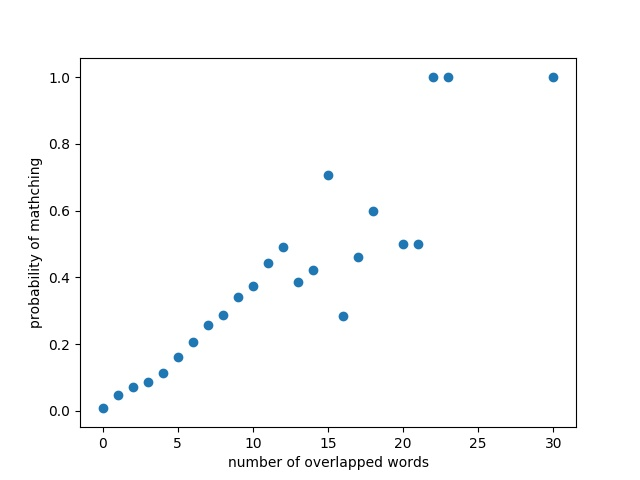
\includegraphics[width=2in]{overlap-words.jpg}
  \caption[width=\textwidth]{The x-axis refers to the number of
overlapped words in both question and answer sentences. y-axis refers to the probabilities of being the target answer.}
\end{minipage}%
\hfill
\begin{minipage}{.45\textwidth}
  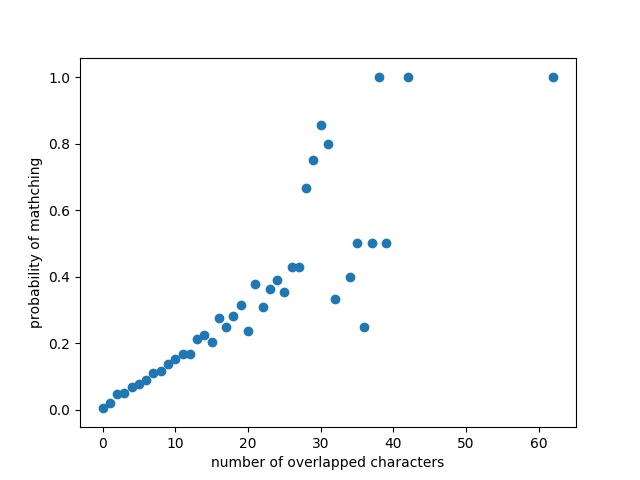
\includegraphics[width=2in]{overlap-characters.jpg}
  \caption[width=\textwidth]{The x-axis refers to the number of
overlapped characters in both question and
answer sentences. While y-axis refers to the
probability of being the target answer.}
\end{minipage}
\end{figure}

\subsubsection{Distance to Question Word}
There are some question words in each question, which indicates the type of question. After statistics, we find 14 questions words(\begin{CJK}{UTF8}{gbsn}
“什么”, “多少”, “多”, “怎样”, “怎么”, “哪里”, “哪”, “谁”, “几”, “啥”, “如何”, “吗”, “何时”, “是否”
\end{CJK}) in total, which cover 8602 of 8772 questions in training data. Fig. 3 shows that in the target answer there are more words near the question word than the distant ones. Thus, intuitively we consider the word closer to the question word as more important one and assign it greater score. Moreover, Fig. 4 shows that the word at the right of the question word is much more than the word at the left. Thus, we will assign greater weight to the word at the right. 

For example, in the question \begin{CJK}{UTF8}{gbsn}
“布卢姆 - 植物 分类学 与 植物 地理学 杂志 每期 有 多少 页 ?”
\end{CJK}, the question word is \begin{CJK}{UTF8}{gbsn}“多少”\end{CJK}. The word closer to the question word is more important, that is \begin{CJK}{UTF8}{gbsn}“每期”, “页”\end{CJK} are most important. (\begin{CJK}{UTF8}{gbsn}“有”, “与”\end{CJK} are regard as stop words and will be removed when data preprocessing). Since we think the word at the right of the question word is more important than the word at the left, we will assign greater weight to \begin{CJK}{UTF8}{gbsn}“页”\end{CJK} than \begin{CJK}{UTF8}{gbsn}“每期”\end{CJK} in this sentence.

\begin{figure}
\centering
\begin{minipage}{.45\textwidth}
  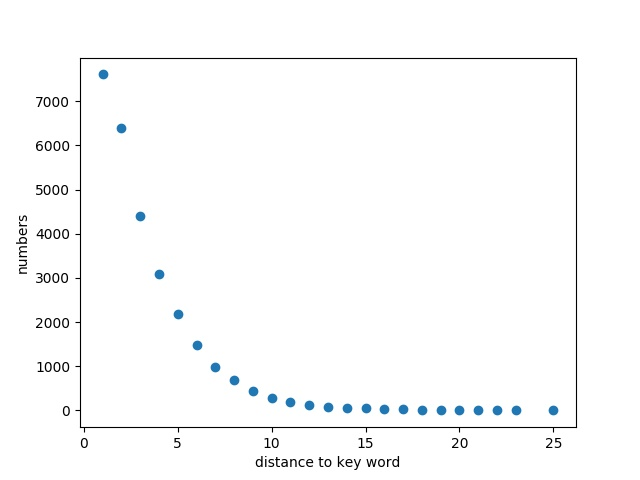
\includegraphics[width=2in]{overlap-distance.jpg}
  \caption{Number of overlapped words over distance. The x-axis refers to the distance from the word in the question to the key-word. The y-axis refers to the number of the words overlapped both in question and the target answer.}
\end{minipage}%
\hfill
\begin{minipage}{.45\textwidth}
  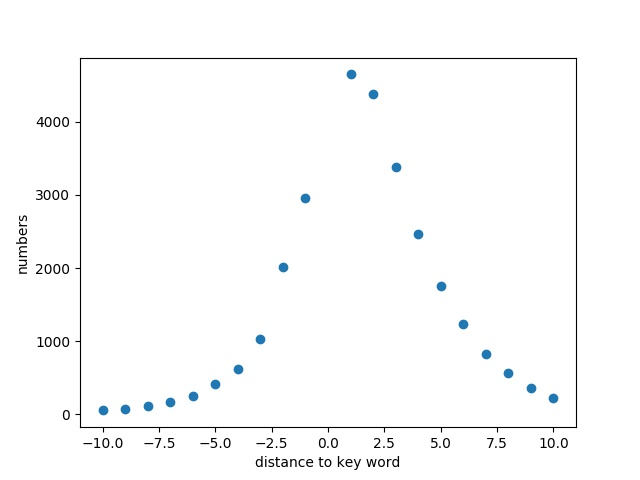
\includegraphics[width=2in]{overlap-distance-all.jpg}
  \caption[width=\textwidth]{Number of overlapped words over distance. The x-axis refers to the distance from the word in the question to the key-word. Positive value means the word is at the right of the key word, while negative means left. The y-axis refers to the number of the words overlapped both in question and the target answer.}
\end{minipage}
\end{figure}



\subsection{Data Preprocessing}
Due to the lack of the obvious boundaries of Chinese, we use the nlpir\footnotemark\ to
segment the Chinese text. Stop words are removed for dropping the useless high-frequency 
words which are not discriminative and have little semantic meaning.


\footnotetext{http://ictclas.nlpir.org/}

\subsection{Distance-Based Scoring}

\begin{enumerate}
  \item \textbf{Segment the question.} After segmenting the question and removing stop words, we get a word list $W$.
  \item \textbf{Find the key word.} There is a key word in each question such as 
\begin{CJK}{UTF8}{gbsn}
“什么”, “哪里”, “多少”
\end{CJK}
 etc. We check whether there is a key word in the question and get its position $d$. If there is no key word in the question, we set the position $d$ to be the length of $W$.
  \item \textbf{Scoring word.} For each word $w_i$ ( key word) in word list $W$, we set its score as follow: 
  \begin{equation}
    s_i = \begin{cases}2^{-|i-d|} & i \ne d \\ 0 & i = d \end{cases}
  \end{equation}
  since we think the word near the key word is more important.
  \item \textbf{Scoring the candidate answers.} For each candidate answer $ans$, the score is obtained by Eq.2 
  \begin{equation}
    score_{ans} = \sum_i^l{\delta_i}
  \end{equation}

  \begin{equation}
  \begin{aligned}
  \delta_i = \begin{cases}s_i & w_i \in ans \\ 0 & w_i \notin ans  \end{cases}
  \end{aligned}
  \end{equation}
  $l$ refers to the length of $W$.
\end{enumerate}

\subsection{Weighted Distance-Based Scoring}

According to whether the word $w_i$ is at the right of the key word or at the left, we update the score computation for the word in $W$ as Eq.4  

  \begin{equation}
  \begin{aligned}
    s_i = \begin{cases} \beta \times 2^{-|i-d|} & i > d \\
     2^{-|i-d|} & i < d \\
     0 & i = d
     \end{cases}
  \end{aligned}
  \end{equation}
$\beta$ is a positive number tuned by training data. In our experiment, $\beta = 4.3$ is optimized.

\section{Experiments}
The provided baselines and our result on training data are showed as Table 1. 
Due to the fact that the above baselines are based on the bag-of-word model
and do not have a learn-based mechanism, the performance is rather poor. 

In our experiments, we combine word
overlap with a distance-based scoring method to rank the candidate answers 
which achieves significant improvement upon baselines.

In the final evaluations of DBQA on NLPCC 2017, our approach gets the MRR of 
0.5571 and ranks 12th among the 21 submissions.
\begin{table}
\centering
\caption{The result on training data}
\begin{tabular}{l@{\qquad}l@{\qquad}l}
\hline\noalign{\smallskip}
Method & MAP & MRR\\
\noalign{\smallskip}
\hline
\noalign{\smallskip}
Machine Translation     & 0.2410 & 0.2412  \\
Average Word Embedding  & 0.4610 & 0.4610  \\
Paraphrase              & 0.4886 & 0.4906  \\
Word Overlap            & 0.5114 & 0.5134  \\
\hline
Distance-based Overlap  & 0.6848 & 0.6874  \\
Weighted Distance-based Overlap   & 0.7266 & 0.7293  \\
\hline
\end{tabular}
\end{table}

\section{Conclusion}

In this paper, we reported details of our approach for the sub-task of
NLPCC 2017 shared task Open Domain Question answering. In our approach,
we applies an distance-based scoring method to rank the answer candidates. Our 
final performance is not so as some deep learning methods, but it is 
fast and simple and greatly outperform the provided baseline. 

%
% ---- Bibliography ----
%
\begin{thebibliography}{5}

\bibitem {Hu}
Hu, B., Lu, Z., Li, H., Chen, Q.,
Convolutional neural network architectures for matching natural language sentences. 
In: Advances in Neural Information Processing Systems, pp. 2042–2050 (2014)

\bibitem {Qiu}
Qiu, X., Huang, X.: Convolutional neural tensor network architecture for
community-based question answering. In: Proceedings of International Joint
Conference on Artificial Intelligence (2015). http://ijcai.org/papers15/Papers/
IJCAI15-188.pdf

\bibitem {Yu}
Yu, L., Hermann, K.M., Blunsom, P., Pulman, S.: Deep learning for answer sen-
tence selection. arXiv preprint arXiv:1412.1632 (2014)

\bibitem {Liu:Qiu:Chen}
Liu, P., Qiu, X., Chen, J., Huang, X., 
Deep fusion LSTMs for text semantic matching. 
In: Proceedings of Annual Meeting of the Association for Computational Linguistics (2016). http://aclweb.org/anthology/P/P16/P16-1098.pdf

\bibitem {Liu:Qiu:Huang}
Liu, P., Qiu, X., Huang, X.,
Modelling interaction of sentence pair with coupledLSTMs. arXiv preprint arXiv:1605.05573 (2016)

\bibitem {Mikolov}
T. Mikolov, K. Chen, G. Corrado, and J. Dean, “Efficient estimation of word
representations in vector space,” Computer Science, 2013.

\bibitem {Wang}
Wang B., Niu J., Ma L., et al. A Chinese Question Answering Approach Integrating Count-Based and Embedding-Based Features[J]. 2016.

\bibitem {Hochreiter}
Hochreiter, S., Schmidhuber, J.: Long short-term memory. Neural Comput. 9(8),
1735–1780 (1997)

\bibitem {LeCun}
LeCun, Y., Bottou, L., Bengio, Y., Haffner, P.: Gradient-based learning applied to
document recognition. Proc. IEEE 86(11), 2278–2324 (1998)

\bibitem {Fu}
Fu, J., Qiu, X., and Huang, X. (2016). Convolutional Deep Neural Networks for Document-Based Question Answering. Natural Language Understanding and Intelligent Applications. Springer International Publishing.


\end{thebibliography}

\end{document}



